In this chapter we will go through how the installations have been analysed and present the findings.  Then we will revisit the theoretical framework and reflect on the generated knowledge from the practical application of the framework.

\section{Systematising the installations}
Over the course of this thesis, my research buddies and I have visited seven exhibitions from 4 local museums in Oslo, (Figure 9.1). Two of the exhibitions took place at the University of Oslo: department of informatics (ifi), as part of the course Tangible Interaction (IN5470). From these museum visits, we have documented 21 interactive installations that make up the data set, see Figure 9.2 for listing of the installations. In the following sections in this chapter, we will see how the theoretical framework has been applied, e.g., Figures 9.2, 9.4, 9.6, to the resulting Findings in Table 9.3, where all the installations are sorted in the same numeric order as in Table 9.2. The framework's practical application also generates three radar charts, where the dimensions/ principles make up the edges of the radar chart, and the numbered lines outward represent the number of installations. E.g. in Figure 9.3, you can see the number of installations starting from 0 in the centre up to 17 outermost. That tell us that of 21 installations in total, 17 of is the highest amount of installations that count that specific dimension/ principle.

\begin{table}[H]
\centering
\begin{tabular}{| l | l| l|}
\hline
\textbf{Type} & \textbf{Name} & \textbf{Museum}\\
\hline
Exhibition & Vi står i det nå & Klimahuset \\
Exhibition & I/O (In Oslo) & Atelier Nord\\
Exhibition & Shadows & MUNCH\\
Exhibition & Poison & MUNCH \\
Exhibition & Input/Output & Teknisk Museum \\
Exhibition & Slow Design: reveal & ifi \\
Exhibition & Haptic Interaction & ifi \\
\hline
\end{tabular}
\caption{Exhibitions}
\label{tab:abc}
\end{table}

\begin{table}[H]
\centering
\begin{tabular}{| l | l | l|}
\hline
\textbf{Nr} & \textbf{Exhibition} & \textbf{Installation}\\
\hline
1 & Input/Output & Input/Output  \\
2 & I/O (In Oslo) & I/O (In Oslo)\\
3 & Slow Design & Qi \\
4 & Slow Design & Memento Mori \\
5 & Slow Design & Presence in existence \\
6 & Haptic Interaction & The Maze \\
7 & Haptic Interaction & Black Horizon \\
8 & Haptic Interaction & The unfair fun fair \\
9 & Vi står i det nå & Crank lever \\
10 & Vi står i det nå & Rotating disc \\
11 & Vi står i det nå & Solutions \\
12 & Vi står i det nå & Video theatre \\
13 & MUNCH & Shadows -- Paint like Munch \\
14 & MUNCH & Shadows -- Resting sofa chair  \\
15 & MUNCH & Shadows -- Camera \\
16 & MUNCH & Shadows -- Edvard M. paints your portrait  \\
17 & MUNCH & Shadows -- Radio \\
18 & MUNCH & Shadows -- Telephone  \\
19 & MUNCH & Shadows -- Suitcases  \\
20 & MUNCH & Shadows -- Housekeeper  \\
21 & MUNCH & Poison  \\
\hline
\end{tabular}
\caption{Installations}
\label{tab:abc}
\end{table}


\section{Application of theoretical framework}
In my attempt to answer how one can design meaningful interactive experiences in a museum space that addresses sustainability, I have accounted for three theories I base my understanding of meaningfulness on; \emph{Hybrid place, place as a dialogue} and \emph{Sense-making strategies}. (My notion is that), together they form the basis to identify meaningful relations between visitor-experience, installation and the museum. The challenge of combining/ putting the three of them together is that we end up with 14 different parameters; e.g. social and cultural dimension from the \emph{Hybrid Place} framework, vs open or relational principle from \emph{Place as a Dialogue}. Which is why it was decided to make table for each theory, where installations is categorised up against the four or five principles. To get a feeling of how the theory applied to the data-set in practise, it was created an additional radar-chart as a complementing way of interpreting the data-set. See section 9.3: Tables and Radar Charts, Figure 9.2-9.7 for the tables and radar charts. This way we could first learn how applicable the different principles/ or dimensions are for the data-set for each of the three theories, and secondly open for seeing connections across/ between the theories; "the bigger picture". The tables later also proved useful as quick-reference guides when mapping out the findings. The categorisation of the data is highly subjective but theoretically grounded, based on my personal experience with- and interpretation of the installations and knowledge of the museum institution the installation was part of. (The plotting of the tables are based upon the written experience accounts and my subjective intuition consisting of both my memory and take-away of the installation.) To begin with I chose to merge all of the MUNCH - \emph{Shadows} installations as one, because I did not think they differed enough in their interactive qualities, and I was afraid that they were going to skew the data. Because of this, the data-set shrinked from 21 to 16. After the first categorisation where the MUNCH \emph{shadows} installations was counted as one, I wanted to compare and see what happened when I categorised each \emph{Shadows} installation. Going through the \emph{Shadows} installations once again, it became clear that they did not all "check the same boxes", which strengthened the decision to count them separately. Then, the data-set increased back to 21 installations again.

\begin{figure}[H]
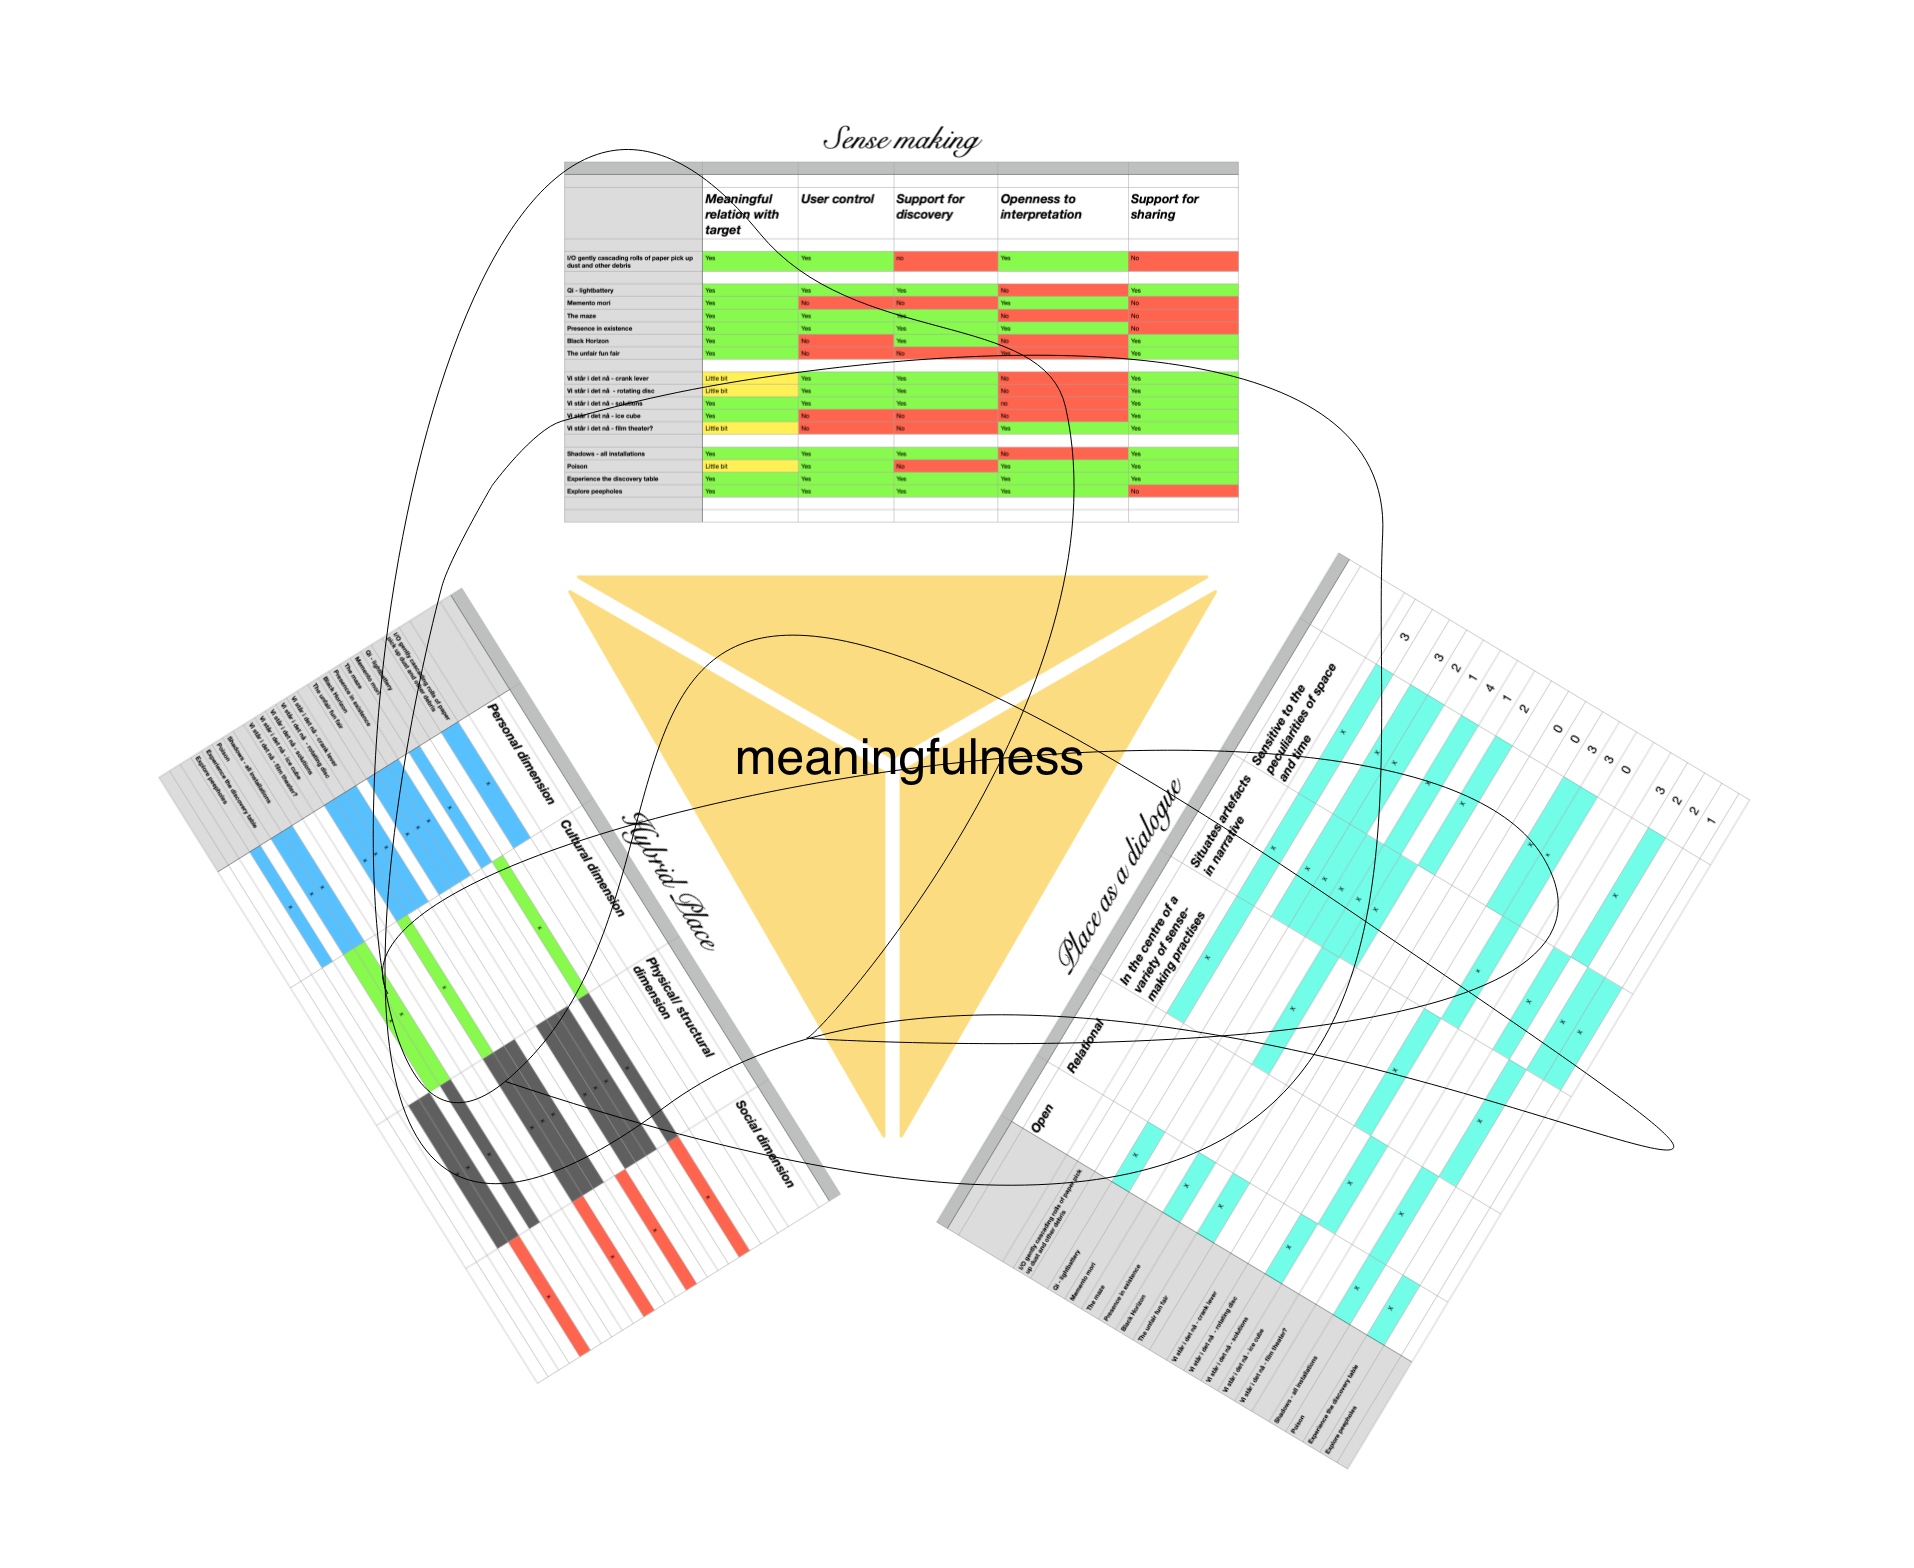
\includegraphics[width=14cm]{pictures/analysis/table_triangle.png}
\caption{Illustrates how each theory contribute to the understanding of meaningfulness. The lines represents what we strive to find; dialogic relations between visitor and installation, and objectifying meaningfulness as a quality that you can design for}
\end{figure}

\section{Tables and Radar Charts}

\begin{figure}[H]
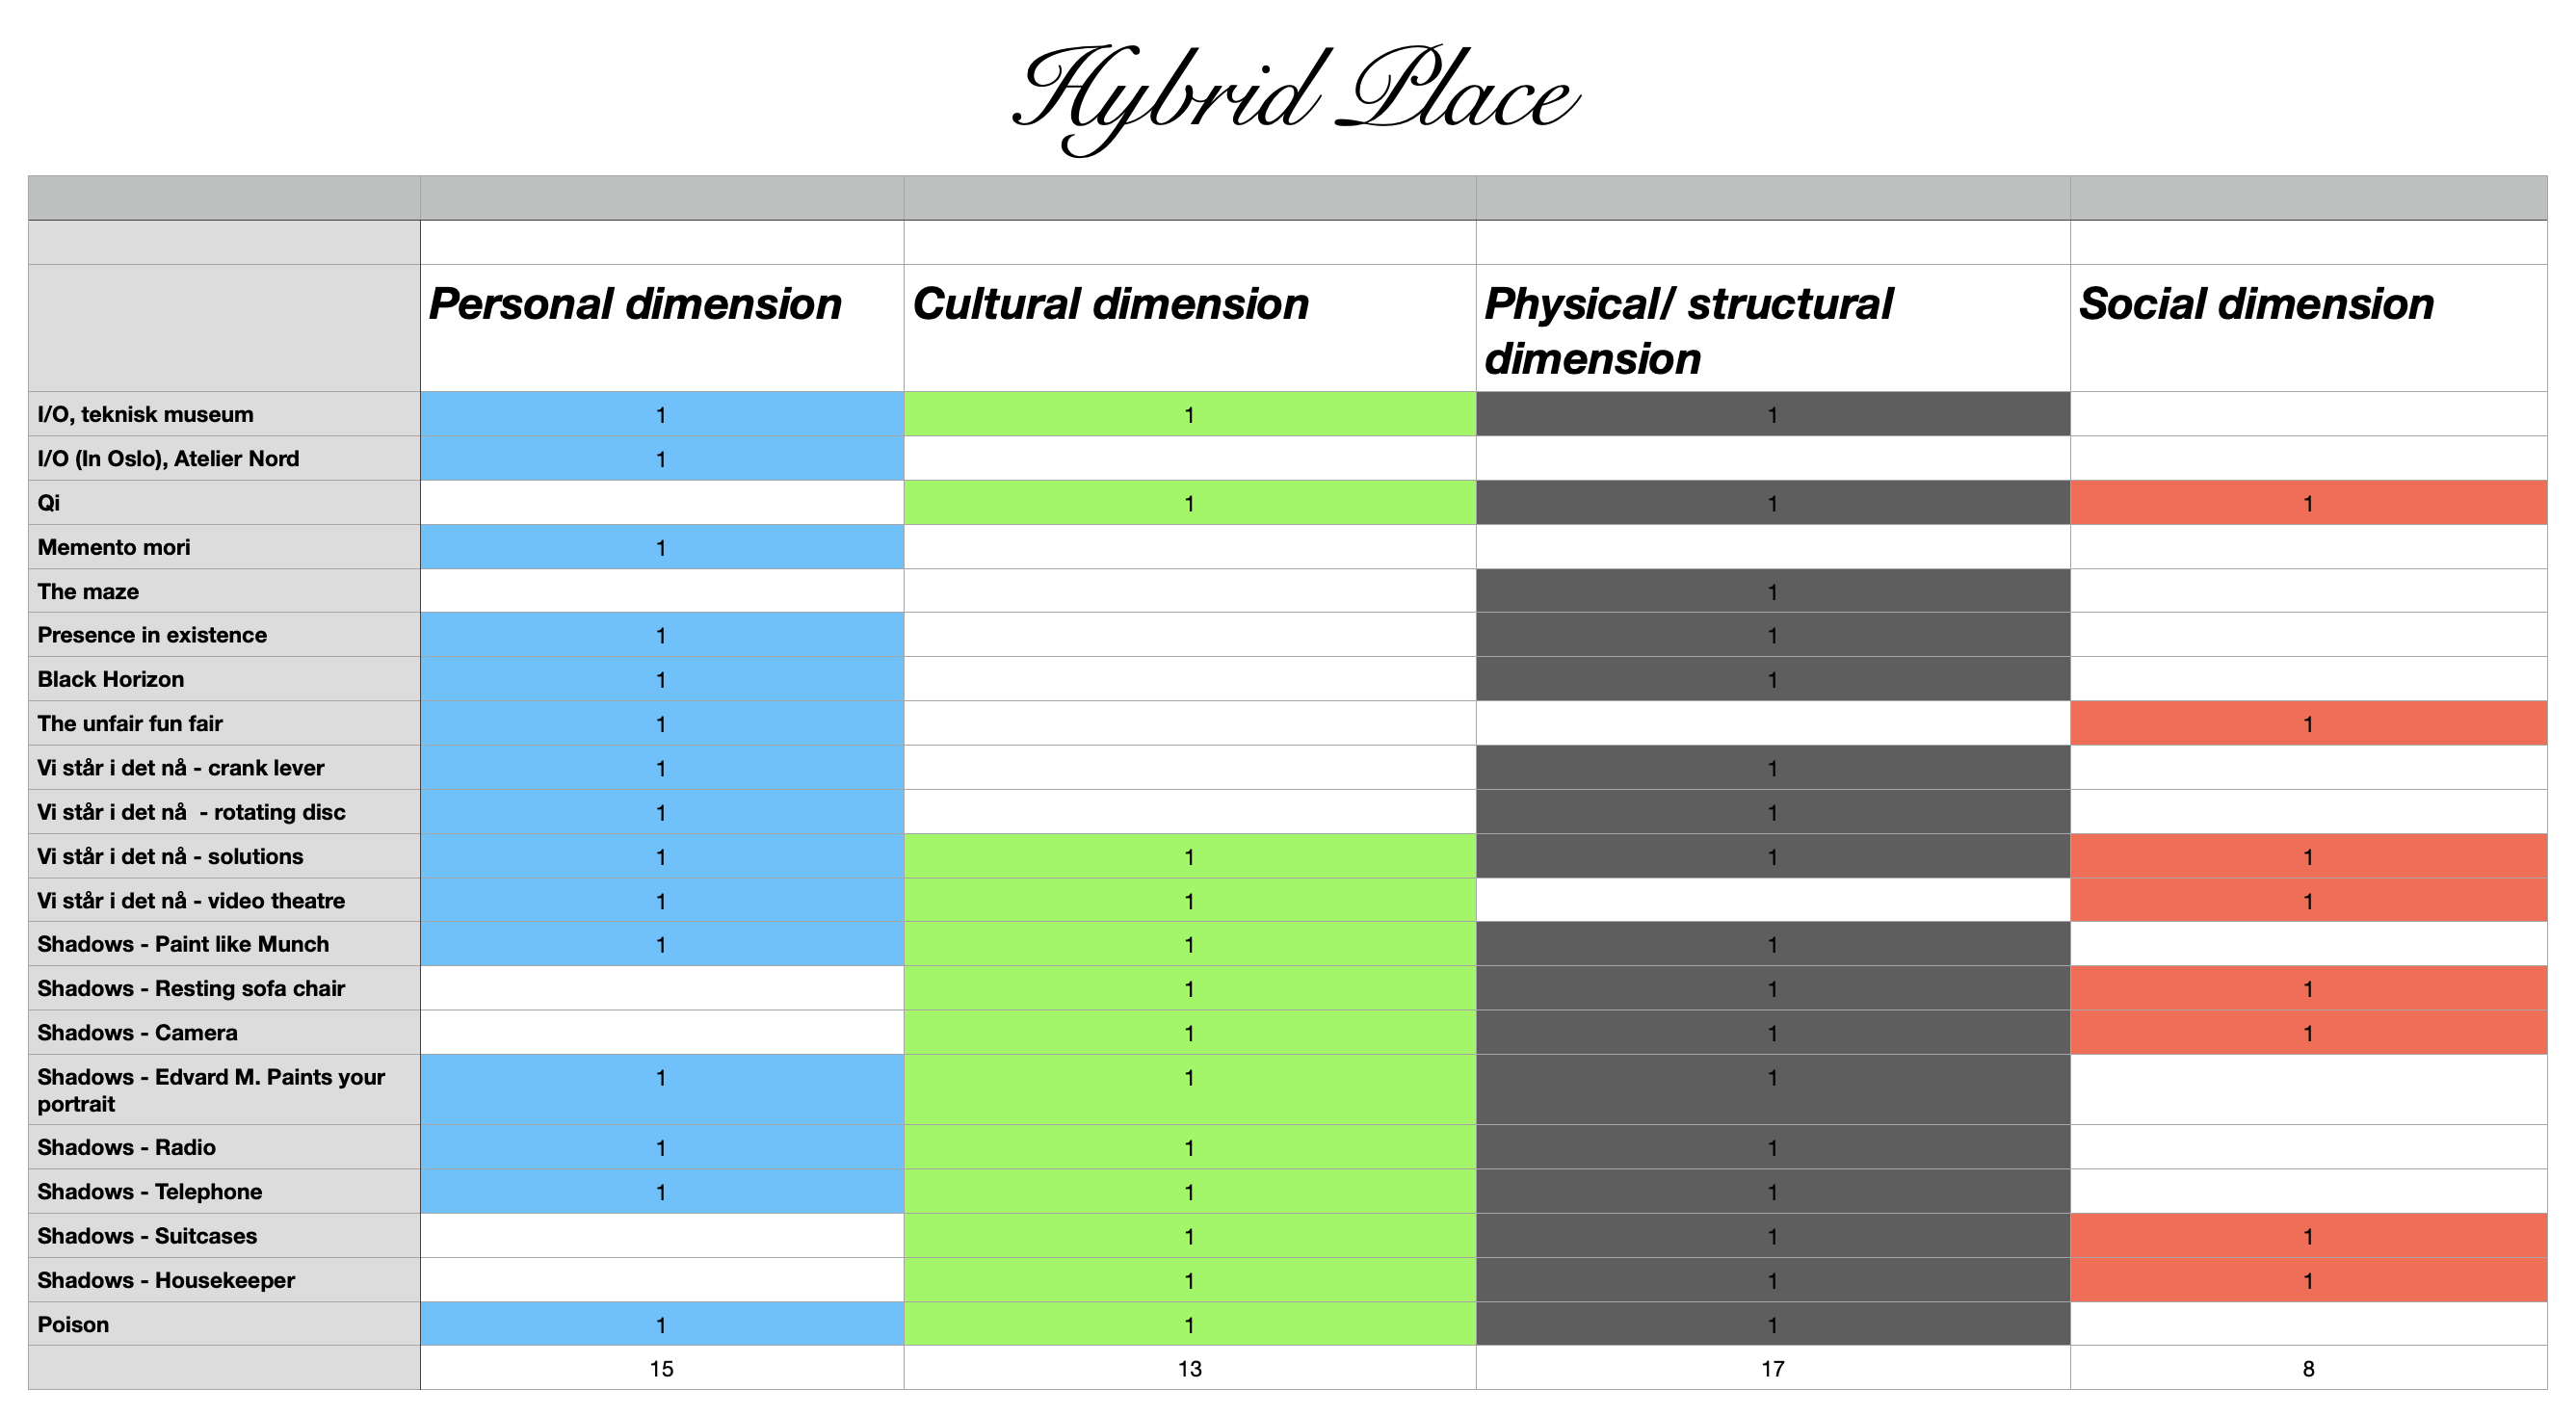
\includegraphics[width=20cm, angle=90]{pictures/analysis/hybrid.png}
\caption{Hybrid Place table}
\centering 
\end{figure}

\begin{figure}[H]
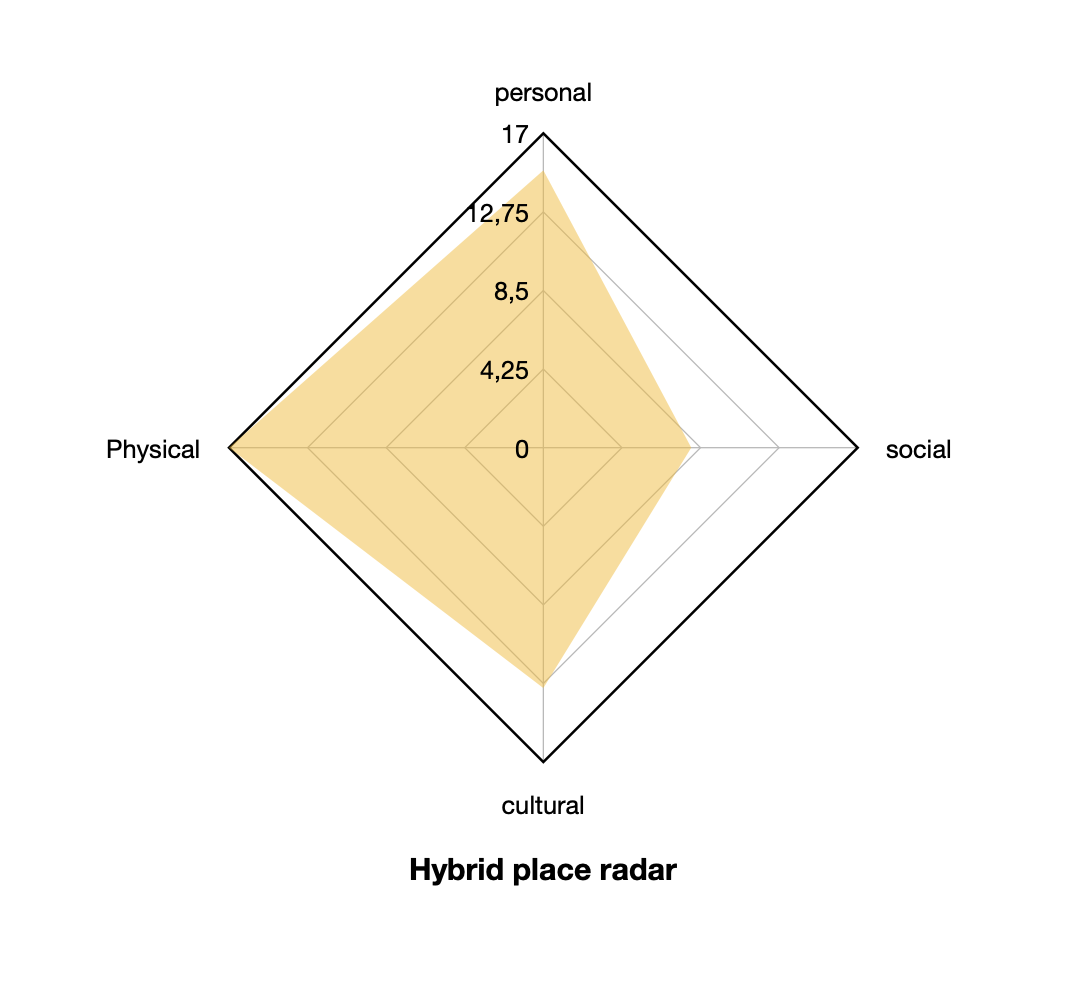
\includegraphics[width=12.5cm]{pictures/analysis/hybrid_radar.png}
\caption{Hybrid Place radar}
\centering 
\end{figure}

From the radar chart we can see that the \textit{Personal} and \textit{Physical} dimension is weighted the most, the \textit{Cultural} dimension less so, and the \textit{Social} dimension the least. Comparing with Figure 9.2, we see that the MUNCH \textit{Shadows} installations account for both the Physical and Cultural dimension results to stand out, whereas all of Shadows marks Cultural and Physical. Looking at the Figure 9.2 again, we can see that the Physical dimension still would be weighted along with the Personal dimension if we were to see MUNCH \textit{Shadows} as one, something which is not the case with the Cultural dimension.


\begin{figure}[H]
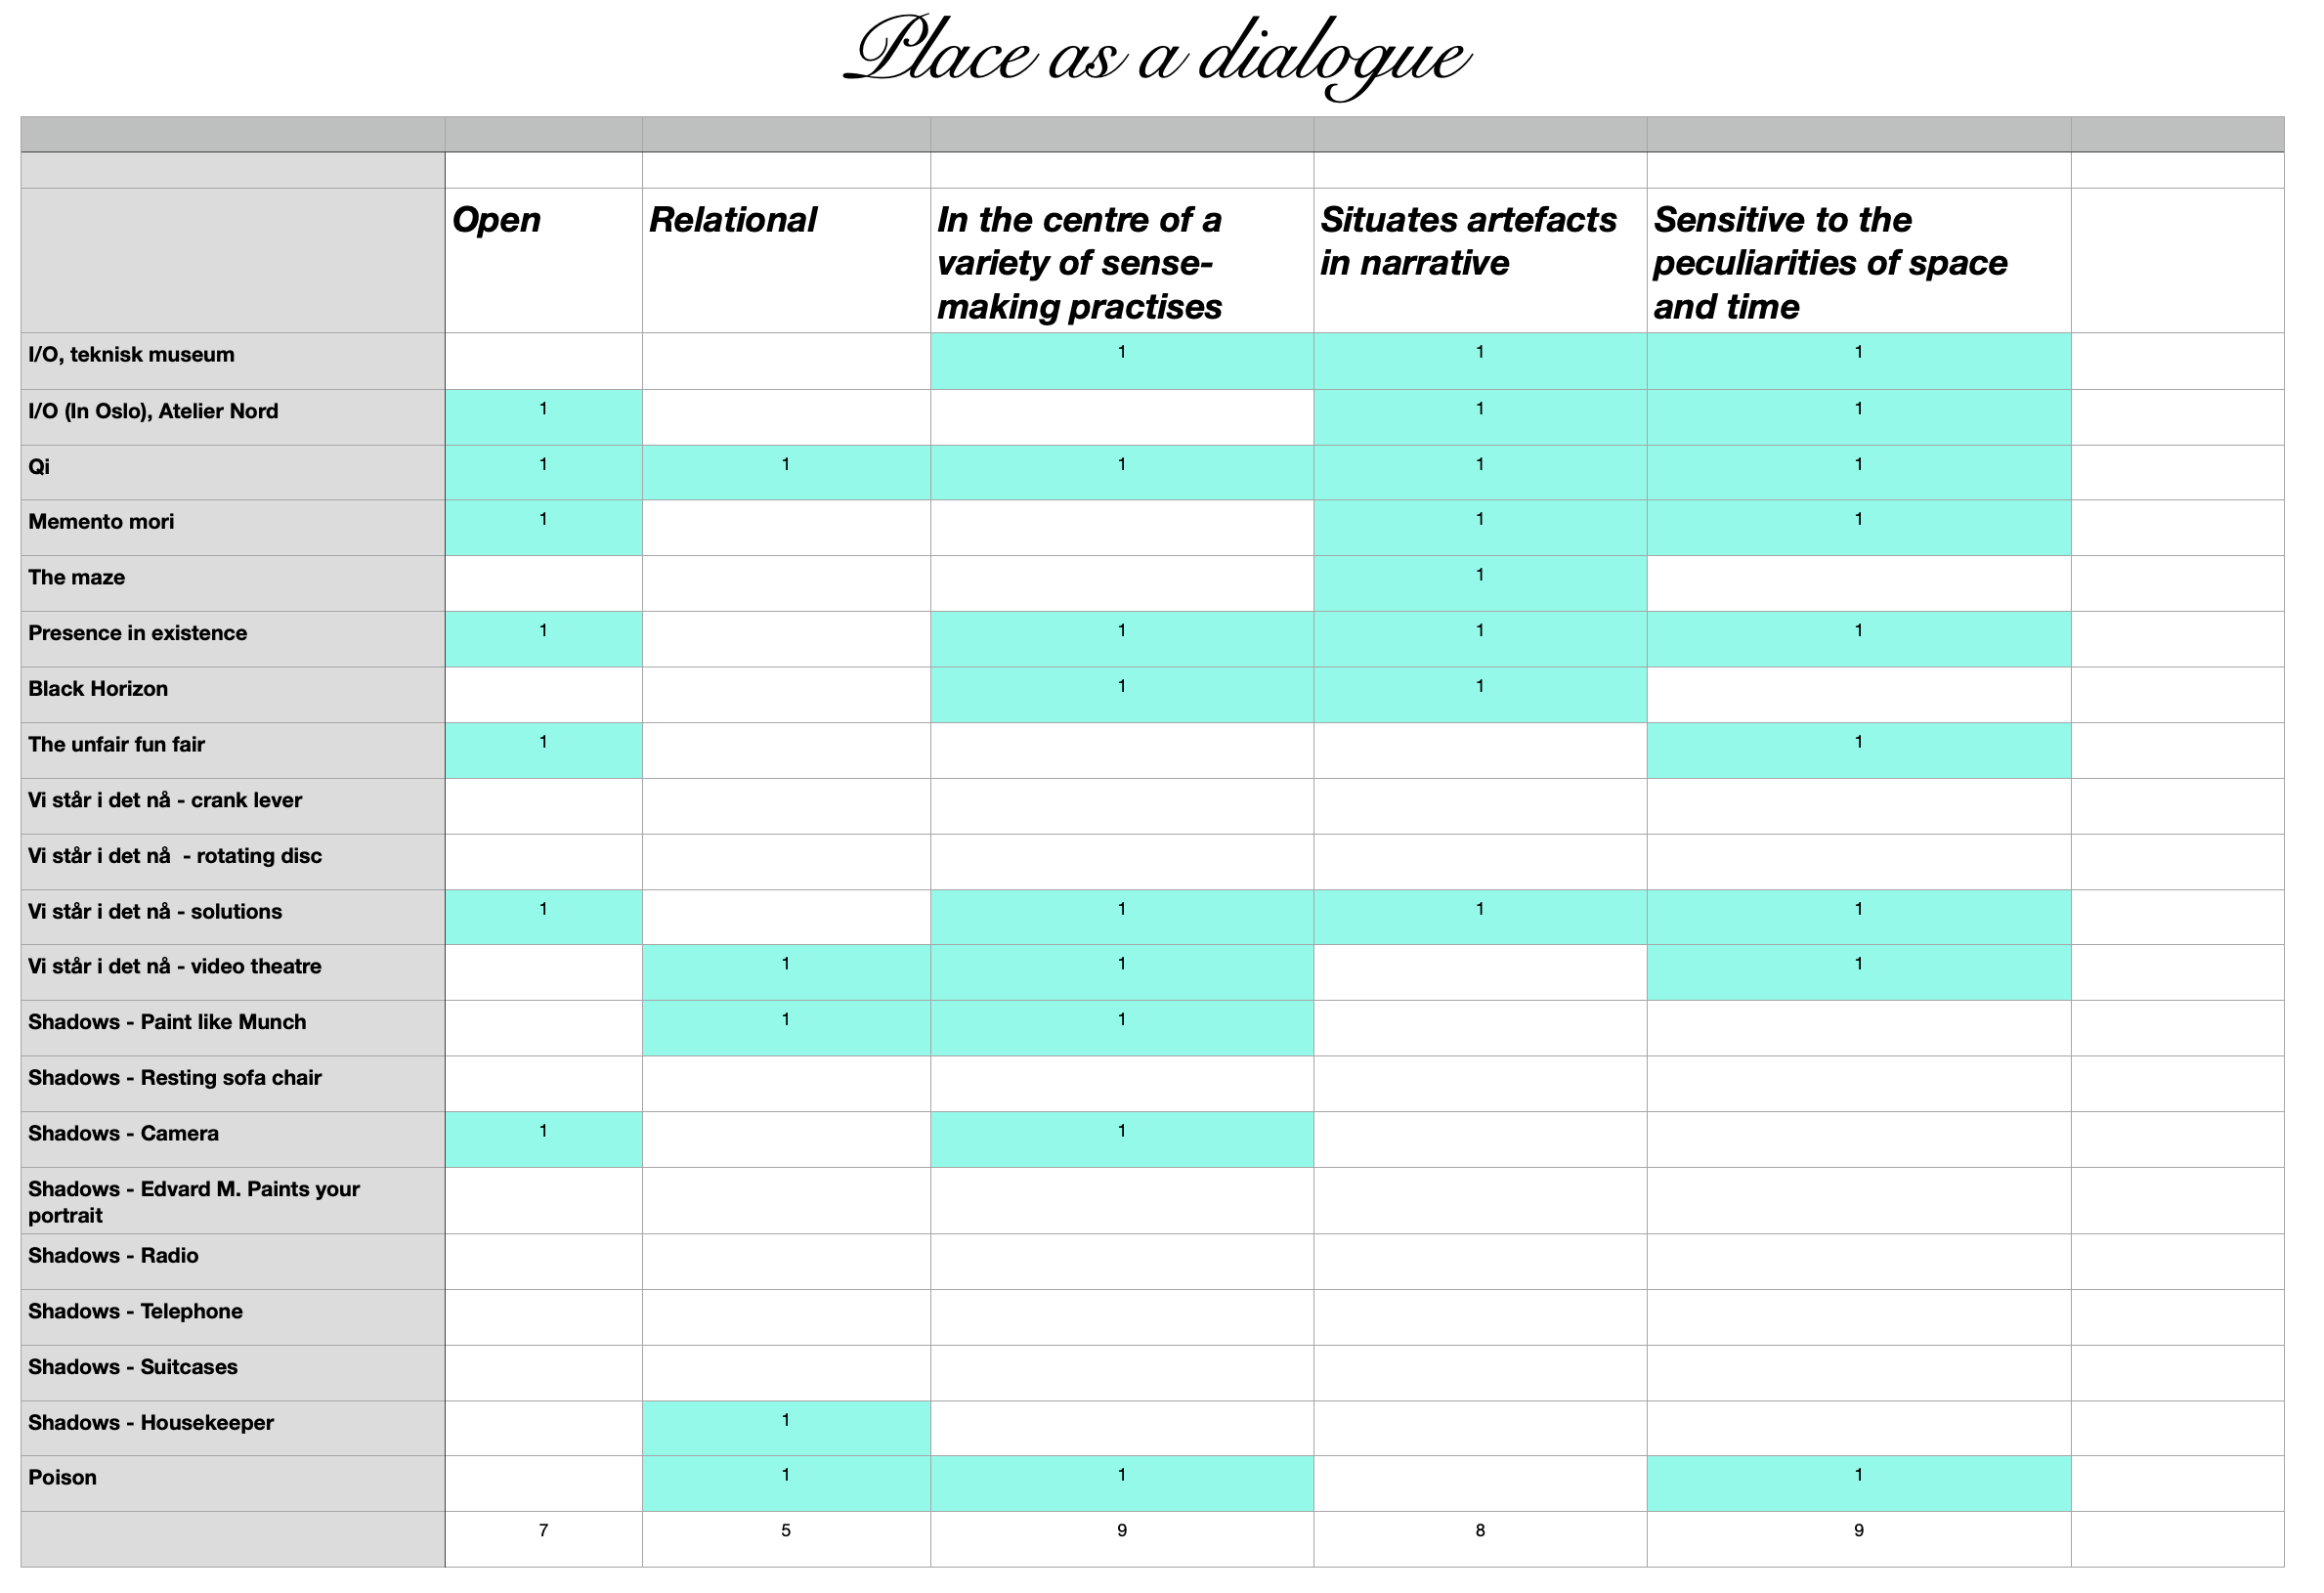
\includegraphics[width=20cm, angle=90]{pictures/analysis/place.png}
\caption{Place as a Dialogue table}
\centering 
\end{figure}

\begin{figure}[H]
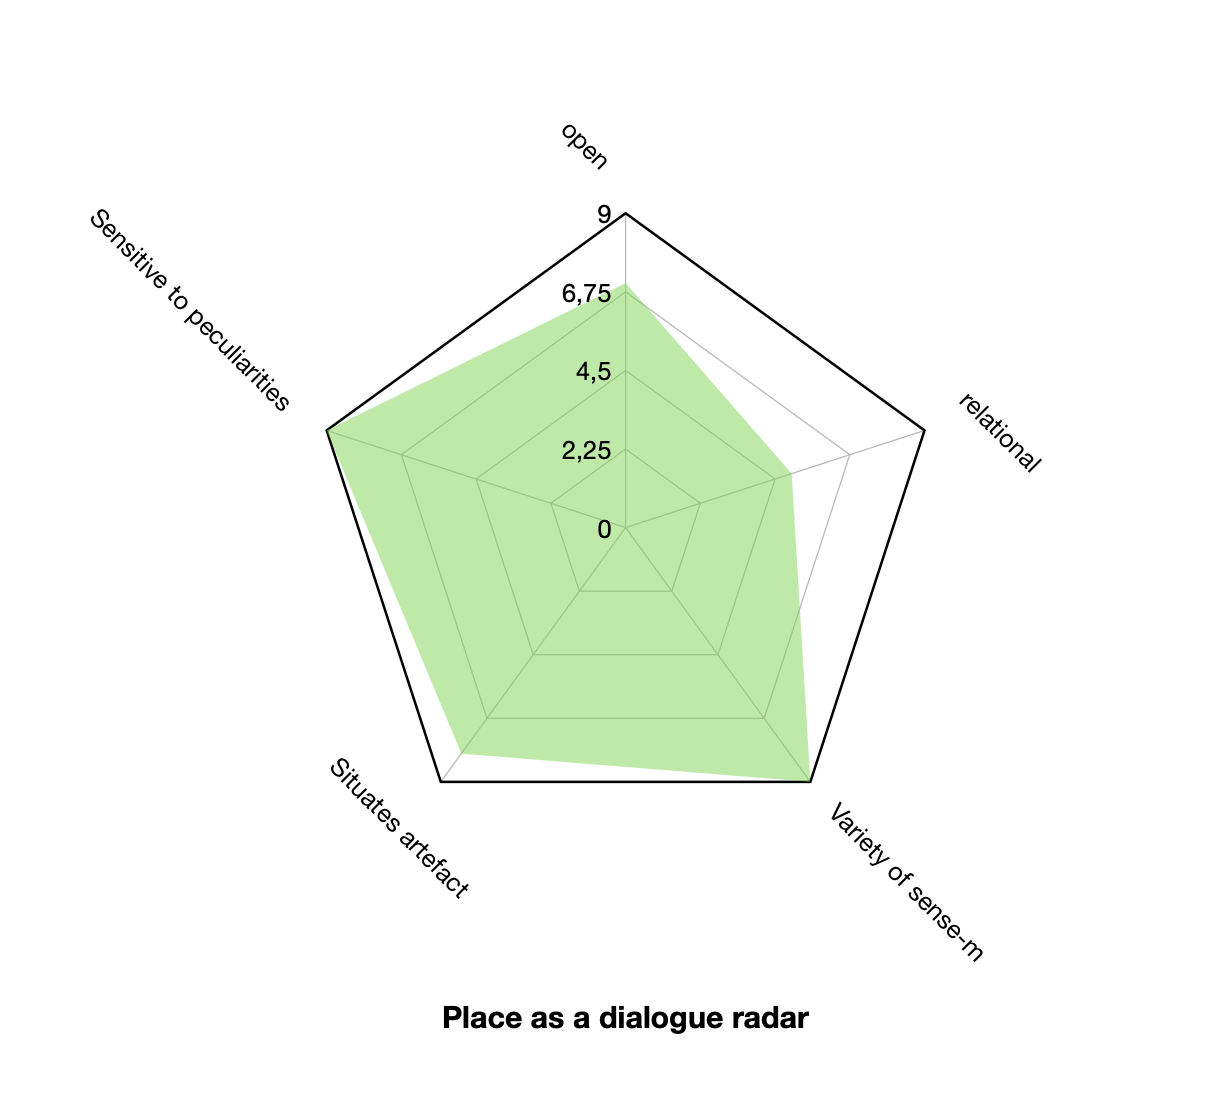
\includegraphics[width=12.5cm]{pictures/analysis/place_radar.png}
\caption{Place as a Dialogue radar}
\centering 
\end{figure}

From the radar chart we can see that the installations point to \textit{Sensitive to peculiarities of space and time}, \textit{In the centre of a variety of sense-making practises}, and \textit{Situates artefact in narrative} as the most fulfilled. While \textit{Open} and \textit{Relational} less so. A flaw with this radar chart is that the outer circle only count to 9 installations. As we can see from Figure 9.4, \textit{Relational} only count three installations. Because of the radar chart's proportions it can seem like more installations are fulfilling each principle - while in reality the chart only represents the trend for about half of the installations in total. 

\begin{figure}[H]
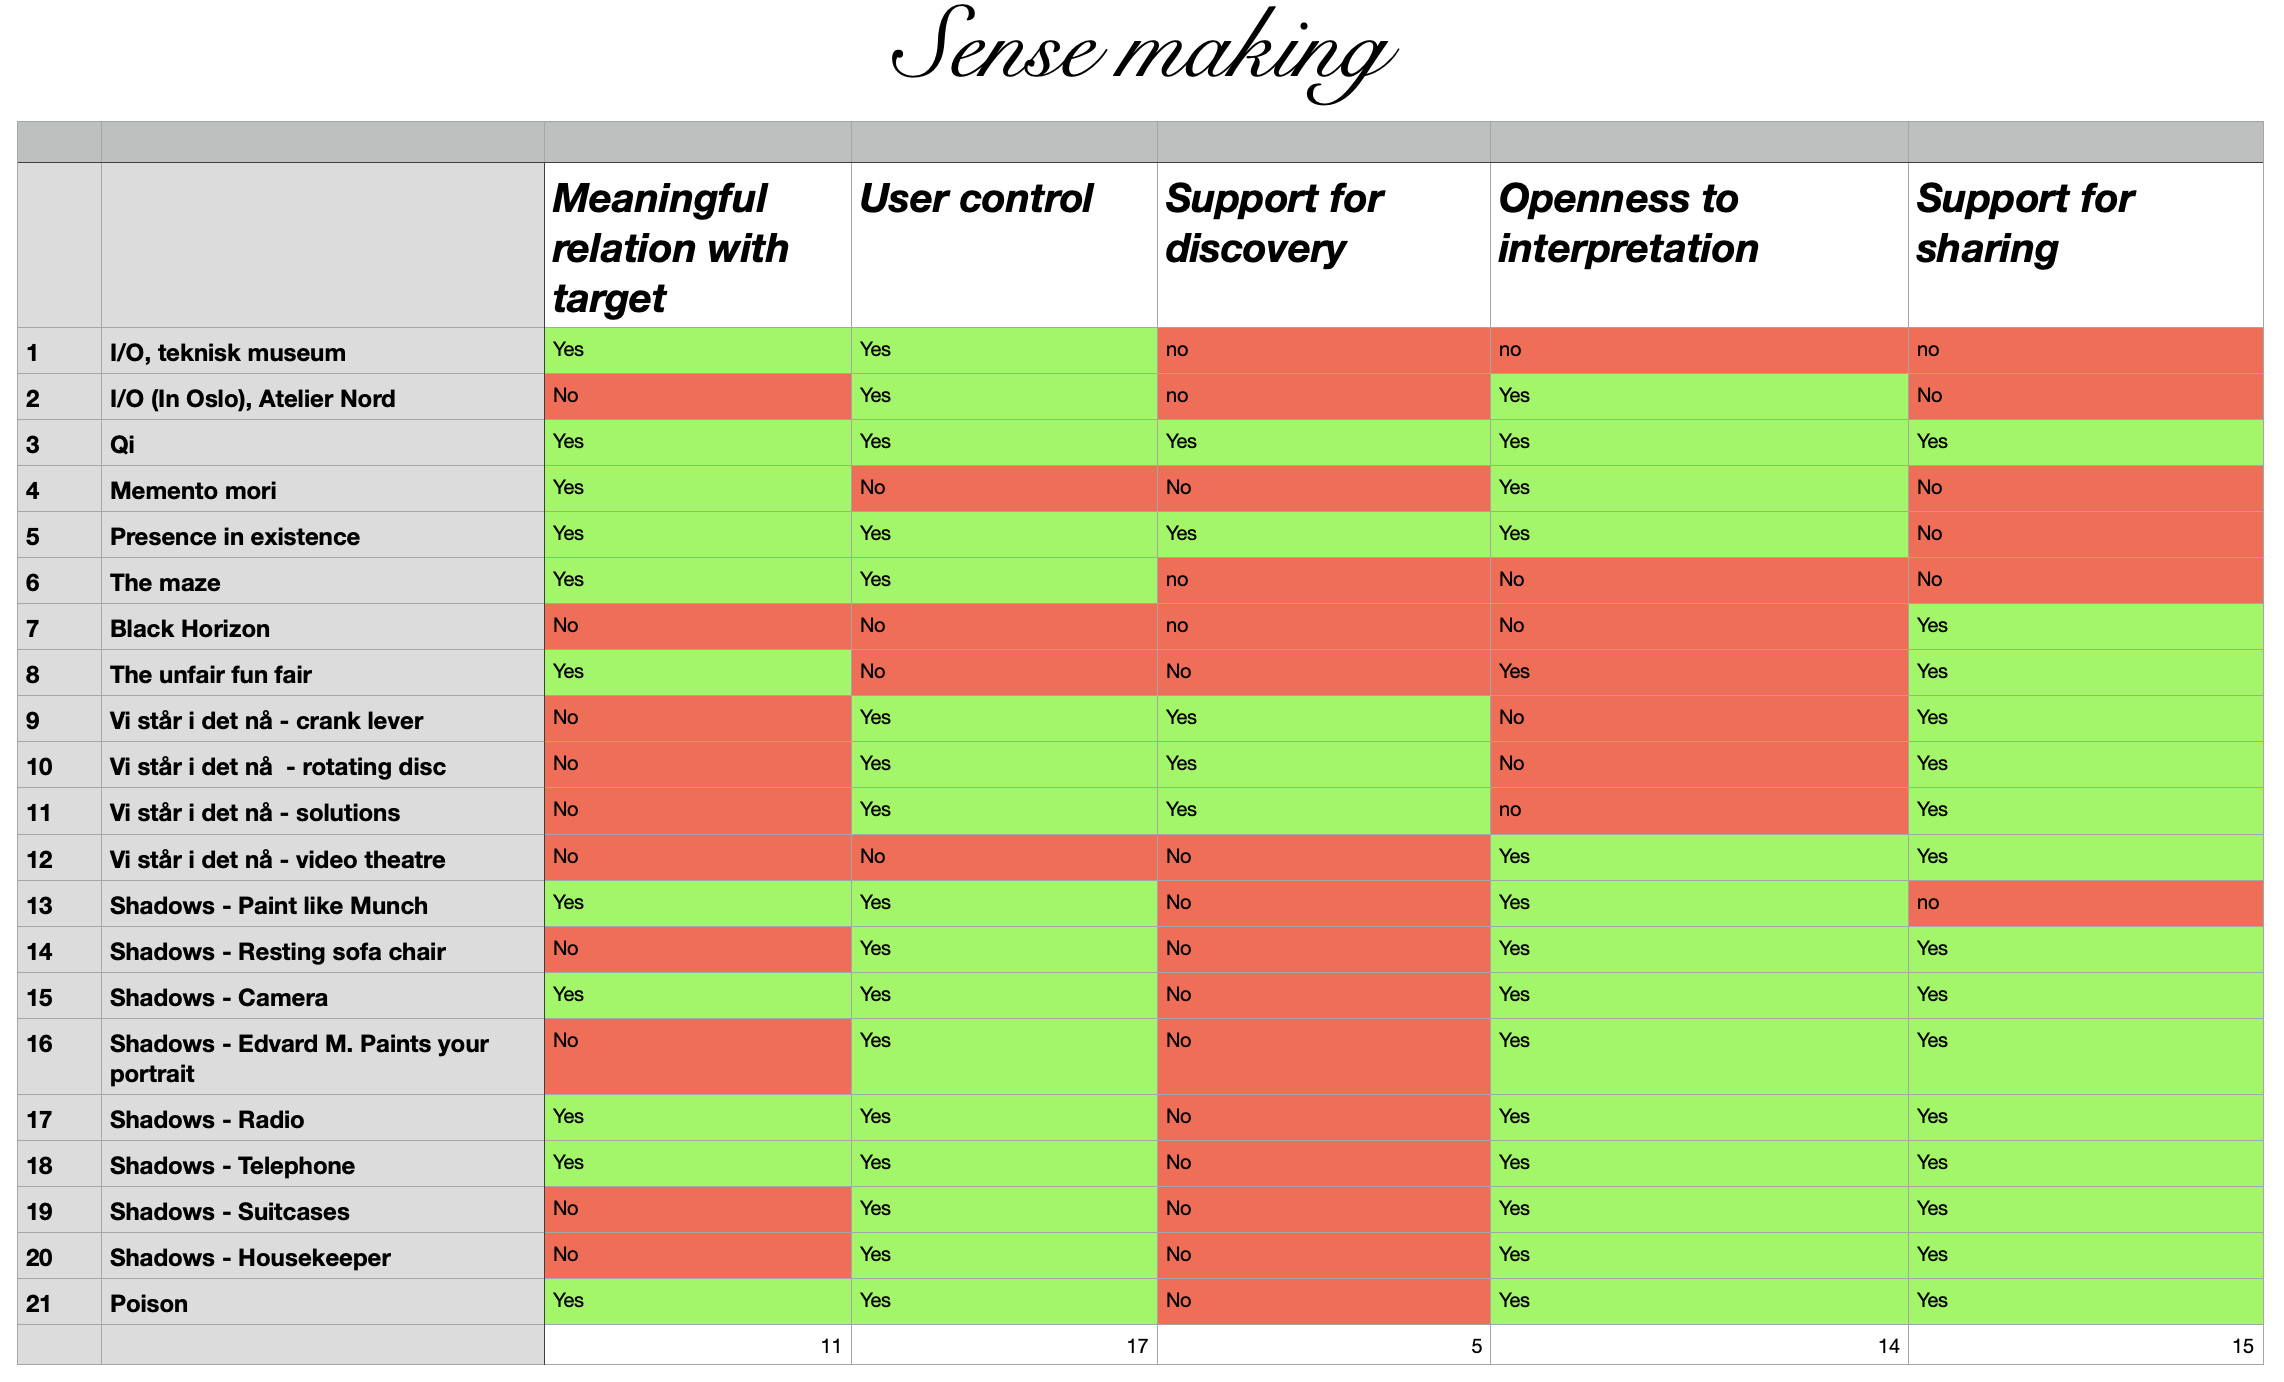
\includegraphics[width=20cm, angle=90]{pictures/analysis/sense.png}
\caption{Sense-making table}
\centering 
\end{figure}

\begin{figure}[H]
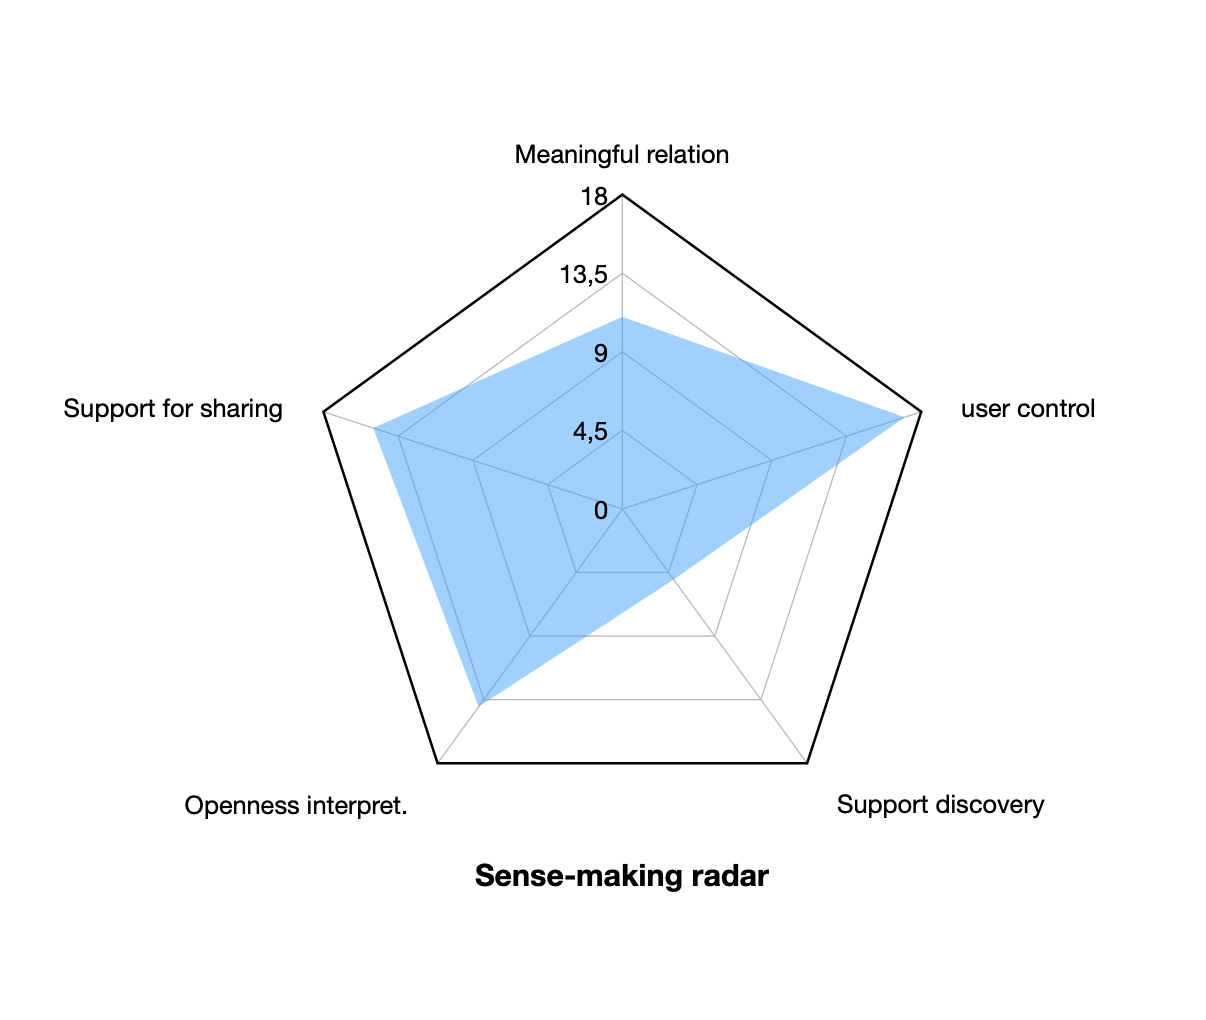
\includegraphics[width=12.5cm]{pictures/analysis/sense_radar.png}
\caption{Sense-making radar}
\centering 
\end{figure}

From the radar chart we can see \textit{User-Control}, \textit{Openness to interpretation} and \textit{Support for sharing} being the most fulfilled, while \textit{Support for Discovery} and \textit{Meaningful Relation} less so. Comparing with Figure 9.6, the validity of \textit{Openness to interpretation} can be misleading stemming from the 9 MUNCH \textit{Shadows} installations which are all marked green - while the rest of the installations in the data-set have more scattered and divided results on that specific principle.


\par
\section{Identifying meaningful relations}
To identify the meaningful relations between visitor-experience, installation and the museum we need to put the three concepts together. As seen at the bottom of Figure 9.2, 9.4, and 9.6, the number of installations adding to the dialogic principle have been counted. This is summarised in Figure 9.8 below in what I have called \emph{Correspondence table}. The number is the amount of installations adding to the principle, e.g. Place open 7, tell us that seven installations qualify to the \emph{Open} dialogic principle from the Place as a Dialogue framework. Figure 9.8 is the first attempt to see how the three theories relates/compares up against each-other. Wanting to see the data-set from a holistic view, abstracting from the details and seeing how the installations map up in the bigger picture.

\begin{figure}[H]
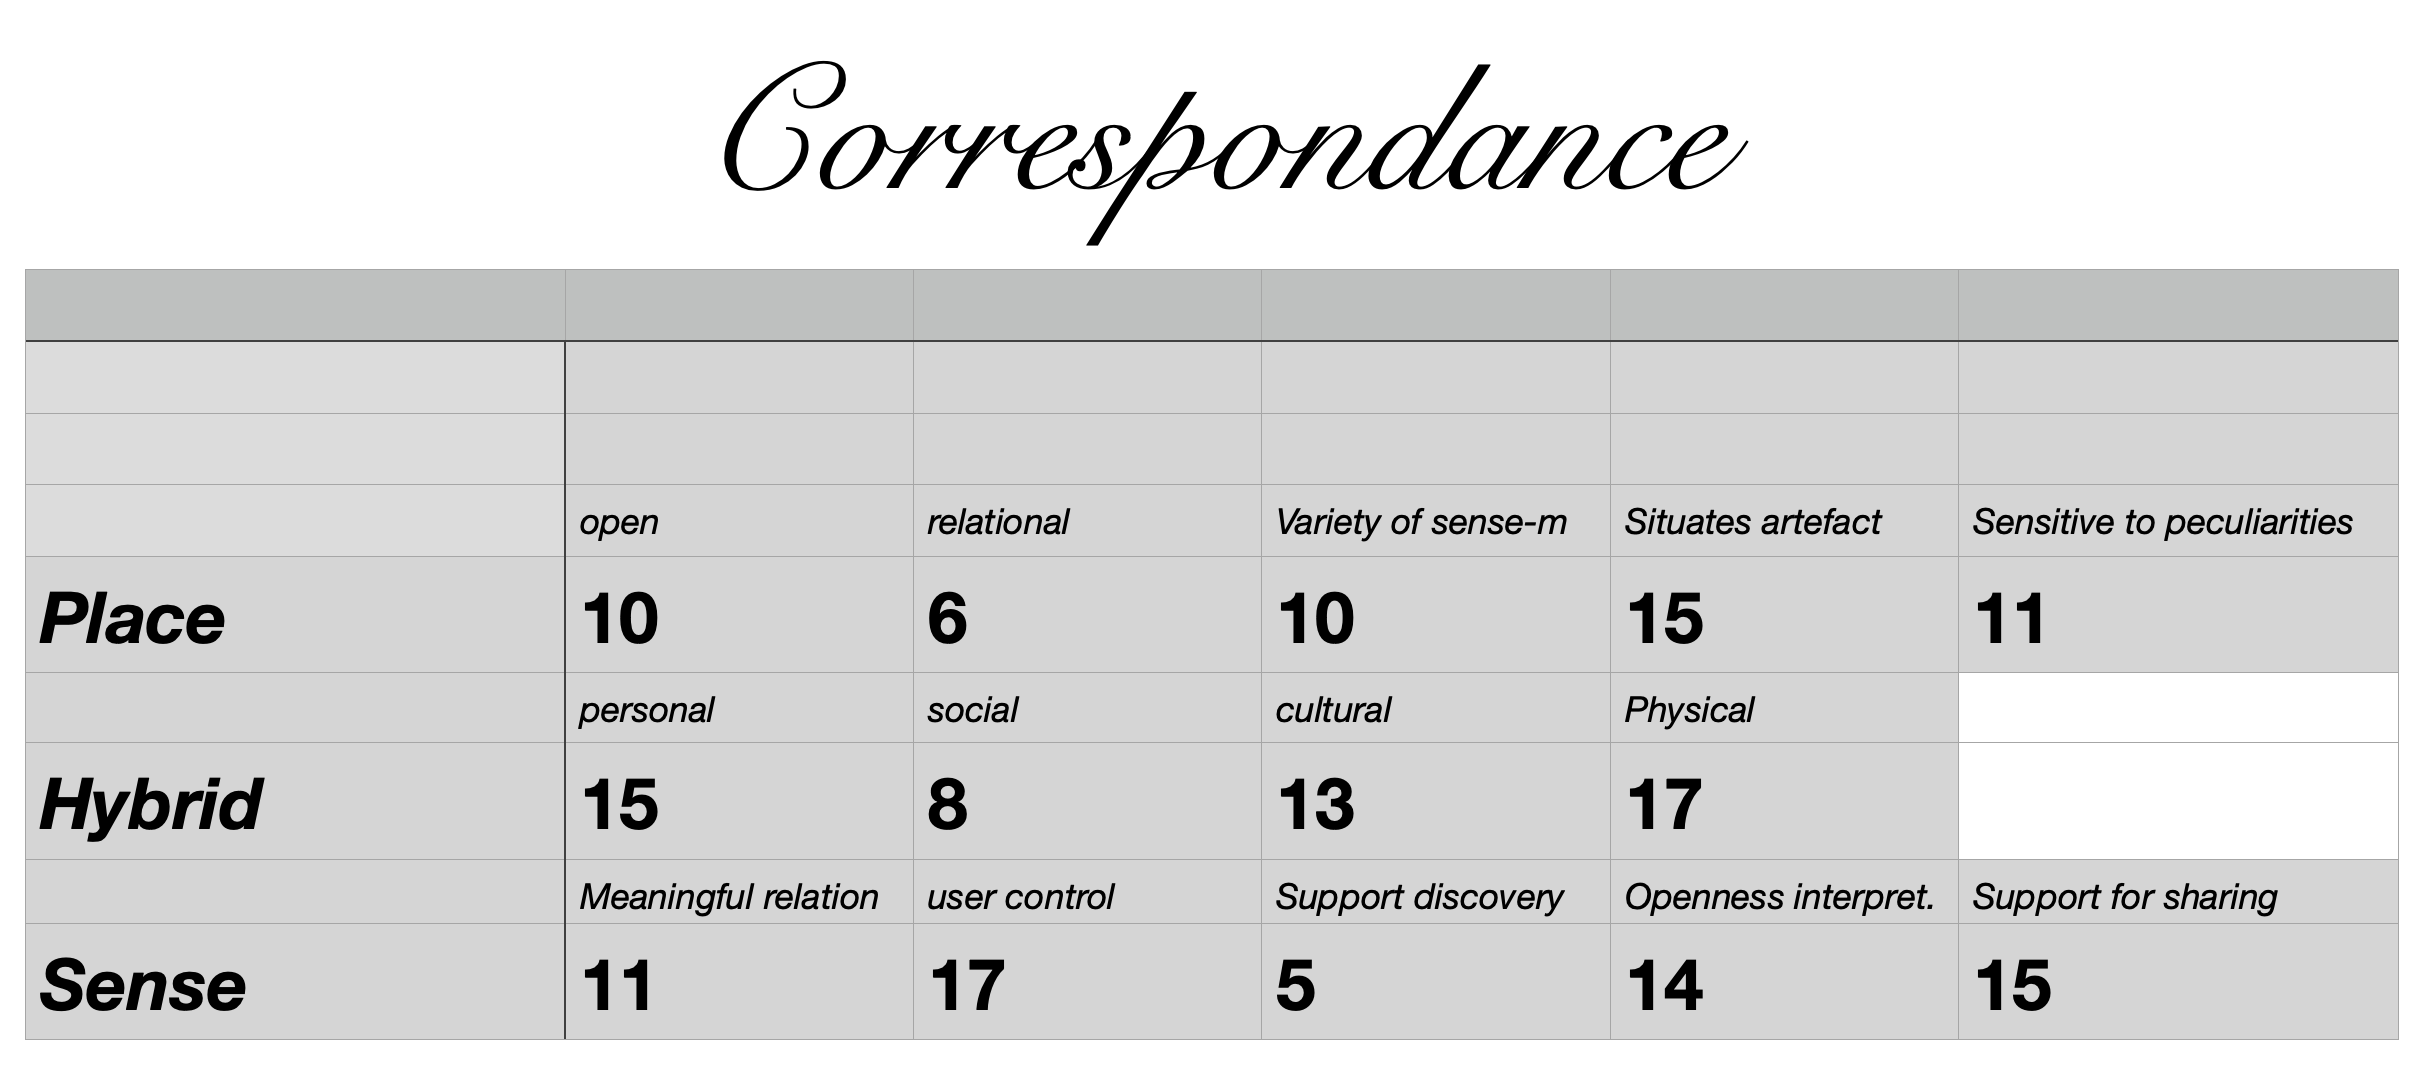
\includegraphics[width=13cm]{pictures/analysis/correspondence.png}
\caption{Correspondence table}
\centering 
\end{figure}

Categorising it this way opened up for looking at the data-set in correlation with each theory separately, while making it possible to see overall trends in the data-set across the theories. One way of doing this would be to highlight the principles with the most installations up against the principles with the least, and it was decided to illustrate this by drawing a heat-map on top of the correspondence table. See Figure 9.9 for the heat-map visualisation. The principles with the highest installation count are coloured in red, then ranging downward from orange to yellow and green, where the blue-colours represents the principles with the lowest installation count.

\begin{figure}[H]
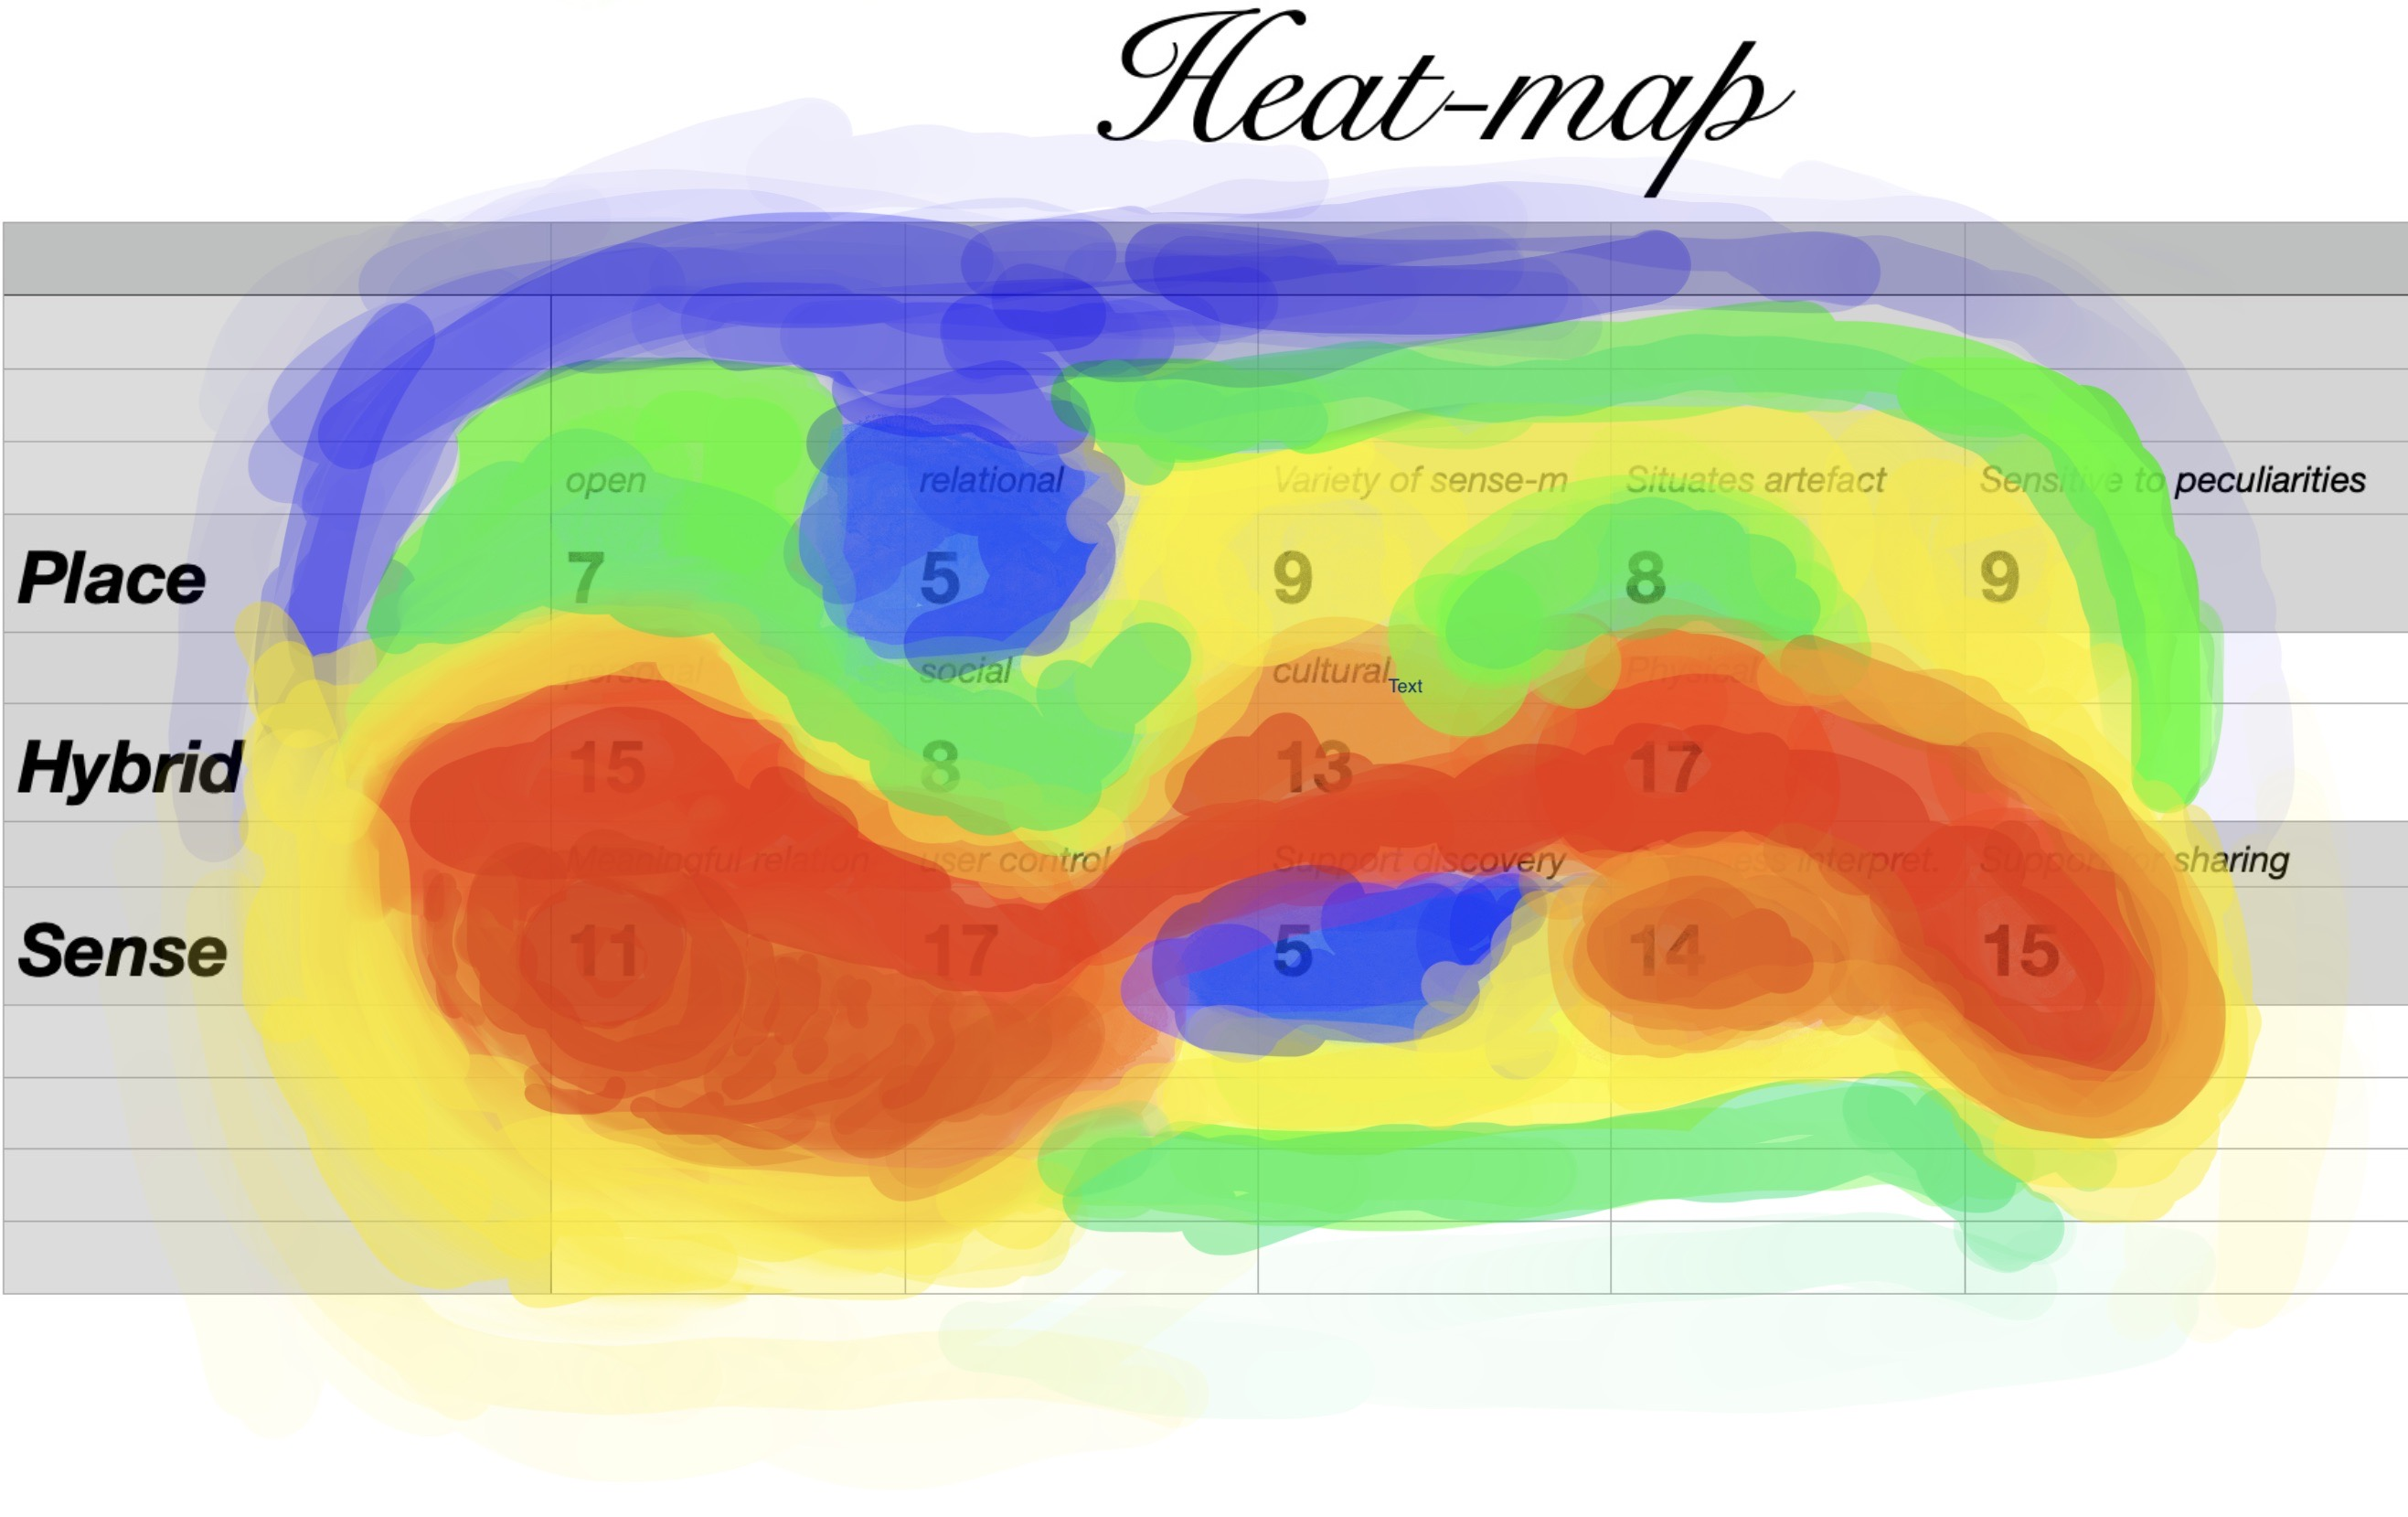
\includegraphics[width=13cm]{pictures/analysis/heatmap.jpeg}
\caption{Heat-map}
\centering 
\end{figure}

What we can see from Figure 9.9 is how well the \textit{Hybrid Place} dimensions intersect and complement the \textit{Sense-making} principles. In Figure 9.5 we notice how the principles only apply to half the data-set. We see the same thing, if not clearer, in the heat-map where the \textit{Place} principles ranges between blue, green and yellow.


\section{Findings}
The main purpose of this analysis-oriented part is to contribute with knowledge that make visible dialogic qualities between interactive installations and visitor-experience. 

"Finally, by making different things intended to address the same problematic situation, RtD can reveal design patterns \autocite{Alexander_book} around problem framings, around specific interactions, and around how theory can be operationalized" \autocite[p. 178]{zimmerman_research_2014}.


"Each one of these patterns is a morphological law, which established a set of relationships in space, which can always be expressed in the same general form: $X \rightarrow r (A, B, ...)$, which means: Within a context of type X, the Parts A, B, ... are related by the relationship r." \autocite[p. 90]{Alexander_book}.


\subsection{Patterns}
In Table 9.3 we present a list of 21 patterns. Each pattern is numbered, and corresponds to the installation numeration in Table 9.2. 

\begin{table}[H]
\centering
\begin{tabular}{| p{0.75cm} | p{1cm} | p{11cm}| }
\hline
\textbf{Nr} & \textbf{H/P/S} & \textbf{Pattern} \\
\hline
1 & S & Presenting an artefact that physically represents the exhibition topic and proposes a personalised route through the exhibition. \\
\hline
2 & S & Leaving the visitor to make its own way through the exhibition space. \\
\hline
3 & S & Having multiple interactive touchpoints with no prescribed sequence of actions, nor a defined start or end. \\
\hline
4 & S & Letting the visitor choose and place an interactive artefact wherever they like on the installation surface to gain access to a personalised end. \\
\hline
5 & S & Having multiple interactive touchpoints with no prescribed sequence of actions, nor a defined start or end. \\
\hline
6 &S &  Letting the visitor control the installation pace. \\
\hline
7 & S & Making the visitor "repair" the installation by putting the interactive elements where they belong, to gain access to the end. \\
\hline
8 &S &  Guiding two-and-two visitors through a prescribed sequence of actions, as a necessity to get the message across.  \\
\hline
9 &S &  Letting the visitor control the pacing of the information display. \\
\hline
10 & S & Gamifying information-claims where the visitor uses a rotating controller to give an answer, as a prerequisite to the information on the topic being displayed. \\
\hline
11 & S & Presenting a token that the visitor can save the choices made during the exhibition to gain access to a personalised ending. \\
\hline
12 & S & Creating a distinct immersive atmosphere through video-projections and sound. \\
\hline
13 & S & Letting the visitor control the pacing of the interactive activity. \\
\hline
14 & S & Recognising the visitors presence, and generating a sound describing the visitor's situational action. \\
\hline
15 & S &  Encouraging the visitor to take a picture of themselves, to become a part of a picture collection related to the installation theme.  \\
\hline
16 & S &  Recognising a visitors presence and action, and telling a story directly to the visitor that nearby visitors can listen in on. \\
\hline
17 & S &  Responding to the visitors action by playing music in the nearby area. \\
\hline
18 & S &  Responding to the visitors action, and telling a story that only the visitor can hear. \\
\hline
19 & S &  Responding to the visitors action, and generating a distinct immersive atmosphere that describes the visitor's situational action.\\
\hline
20 & S &  Recognising the visitors presence, and playing a video where a character speak directly to the visitor. \\
\hline
21 & S & Creating a distinct immersive atmosphere through video-projections and sound.  \\
\hline
\end{tabular}
\caption{Findings}
\label{tab:abc}
\end{table}

\section{Revisiting the framework}
I will now revisit my framework and learn from the analysis where I applied the framework. The framework presented in Chapter 6: A new way of designing for meaningfulness? was built on theoretical understanding from three different approaches to place-centered design. With the knowledge generated from the practical application of the framework when analysing the interactive installations and seeing the resulting list of patterns, I can go back and review the framework with the practical understanding from doing the analysis. Before I introduce the revised version, I will begin by explaining the specific changes I have made to the framework based on the knowledge generated from the analysis.

\subsubsection{From meaningful to dialogic relations}
\subsubsection{}


\section{Revised framework}

present the final theoretical contribution of this thesis: i.e. a framework for identifying dialogic relations between interactive installations and visitors.